\chapter{Teori} %HUSK KILDER
\section{Længde- og breddegrader}
I et geografisk koordinatsystem, er jorden inddelt i længde- og breddekredse. Idet jorden er rund, er disse længde- og breddekredse målt i grader, og de bliver i stedet kaldt længde- og breddegrader. \newline
Længdegrader beskriver de vertikale linjer på verdenskortet i figur 5.1, som går fra nordpolen til sydpolen. Disse bliver også betegnet som meridianer. Meridianen der går gennem Greenwich kaldes nulmeridianen, hvorefter den første vestlige længdegrad bliver udtrykt som 1 grad vestlig længde, og det samme gælder for den første østlige længdegrad, som vil være 1 grad østlig længde. Disse længdegrader bliver herefter talt op, i hver deres retning. Idet en cirkel er 360 grader, er de sidste meridianer på hver sin side af verdenskortet kaldet 180 grader østlig/vestlig længde, da 180 er det halve af 360. Det skal desuden også nævnes, at længdekredsene ikke nødvendigvis har den samme afstand, da længdekredsene har mindre indbyrdes afstand jo tættere på polerne de er. \newline
Breddegrader beskriver de horisontale linjer i verdenskortet nedenunder. Disse linjer er parallelle med ækvator, og deres indbyrdes afstand bliver derfor hverken mindre eller større, men deres omkreds bliver kortere alt efter hvor tæt på polerne de befinder sig.
\begin{figure} [h]
	\centering
	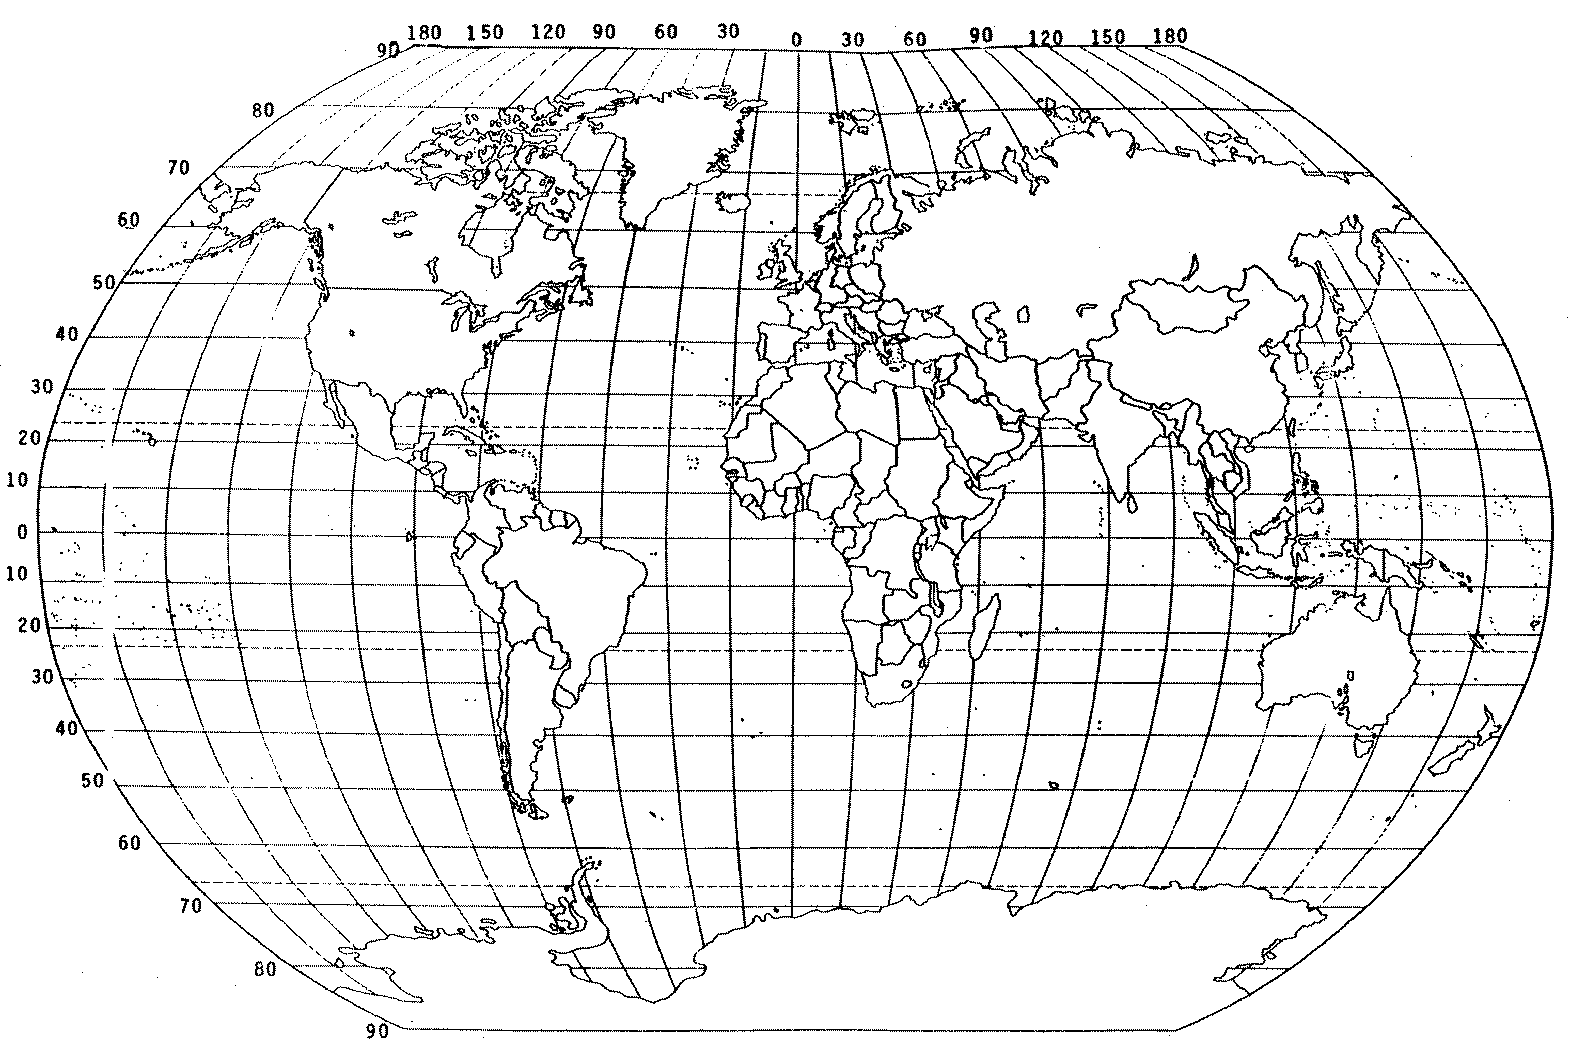
\includegraphics[width=.5\textwidth]{billeder/longlatmap}
	\caption{Verdenskort med længde- og breddegrader}
\end{figure}

Når der ønskes fundet en lokalitet vha. længde- og breddegrader, er det meget simpelt, den længdegrad der bliver oplyst, skal man først finde på verdenskortet, hvorefter den oplyste breddegrad skal findes. Når begge er fundet, er den ønskede lokalitet fundet. Et simpelt eksempel kunne være, at byen Aalborg ønskes fundet, vha. længde- og breddegrader. Ved at benytte Danmarkskortet nedenunder på figur 5.2, kan det aflæses, at Aalborg tilnærmelsesvis har koordinaterne 57\textdegree N og 10\textdegree E. Hvis disse koordinater ønskes meget præcist, er der diverse muligheder online, som Google Maps og lignende der kan aflæse dette meget præcist, ellers skal der anskaffes et kort i mindre målestoksforhold, over f.eks. Nordjylland eller endnu mindre.  
\begin{figure} [h]
	\centering
	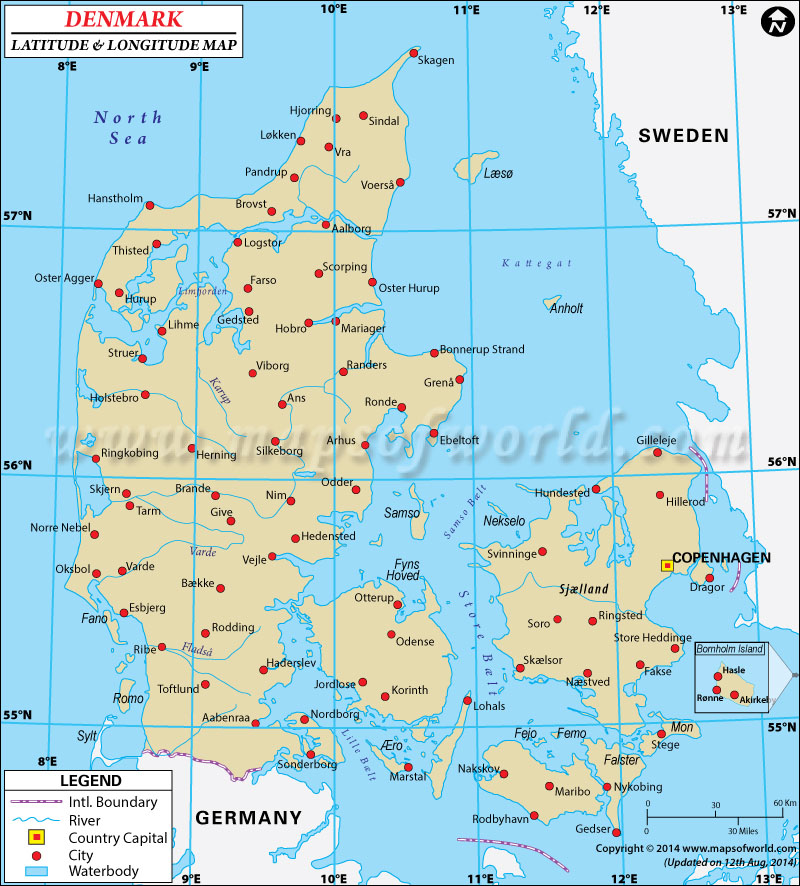
\includegraphics[width=.4\textwidth]{billeder/long-lat-denmark}
	\caption{Danmarkskort med længde- og breddegrader}
\end{figure}

\section{Universal Transverse Mercator systemet}

Universal Transverse Mercator systemet, forkortet UTM, er en måde at opdele jordkloden på, og dermed udforme koordinatsæt for, hvor noget befinder sig henne. Denne metode gør brug af, at jordkloden, som reelt set er rund, bliver omformet til en flade, ligesom et stykke papir. Her bliver jorden inddelt i 60 zoner, hvor hver zone er opdelt fra øst til vest, med numre, og syd til nord med bogstaver. De østlige og vestlige, startende fra 180 meridianen, regnes fra vest til øst med 6\textdegree mellemrum, enkelte zoner er dog blevet gjort bredere eller smallere. Hver zone er nummereret efter deres placering i forhold til deres placering fra vest.\newline
Nordligt og sydligt er inddelt mellem 80\textdegree S bredde, og 84\textdegree N bredde, med en afstand på 8\textdegree, udover en enkelt zone der er 12\textdegree. Hver zone er  navngivet ved et bogstav, fra C-X, startende med C i den sydligste zone.
Alle zonerne i UTM systemet er baseret på en Transverse Mercator projektion, som ikke vil blive yderligere beskrevet i denne rapport, hvor en region kan kortlægges uden stor forvrængning af jordklodens ellers runde form. Hvis jorden blev kortlagt i én stor region, vil dette forårsage store afstandsfejlberegninger, da der ikke vil blive taget højde for jordklodens runde form. Det er her at Transverse Mercator projektionen er smart, da den sørger for en lav grad af forvrængning, da det er smalle breddegrader (6\textdegree) der typisk anvendes til zonerne. \newline
Ved positionering gennem UTM systemet, oplyses følgende: Først en zone fra UTM, som f. eks. 17T. Dernæst en østlig og en nordlig afstand. Den østlige udregnes ud fra den centrale median. Den centrale median er en linjen vinkelret på ækvator som går igennem midten af zonen. Denne er sat som 500.000 m østlig for at undgå negative tal, dvs. et punkt vest for medianen giver et tal under 500.000 m, hvor et tal øst for vil være over 500.000 m.  Den nordlige afstand beregnes på følgende måde: Hvis punktet er på den nordlige halvkugle, beregnes den nordlige afstand som afstanden til ækvator. Hvis punktet er på den sydlige halvkugle, beregnes den nordlige afstand som 10,000,000 m minus afstanden til ækvator, for at undgå negative tal.

\subsection{Konvertering}
Som beskrevet i afsnittet løsningsstrategi, er en konvertering mellem længde- og breddegrads systemet til UTM systemet nødvendig. Dog er udregningen ret kompleks og gruppen har derfor valgt ikke at redegøre for formlen i dette teoriafsnit.

Udover konverteringen fra længde- og breddegrads systemet til UTM, skal en konvertering fra UTM til pixels også bruges i projektet. Dette sker ved brugen af en world file. World filen bruges til at oversætte UTM koordinater til pixels på kortet, så det GPS data der loades ind, kan findes på kortet. Dette projekts world file ser således ud:
\begin{description}
\item[mpx] 0.84964441
\item[roty] 0.00000000
\item[rotx] 0.00000000
\item[mpy] -0.84964441
\item[x0] 539276.35483168
\item[xy] 6250863.73506770
\end{description}
mpx - Antal meter pr pixel i x-retning\newline
roty - Rotationsværdi om y-aksen\newline
rotx - Rotationsværdi om x-aksen\newline
mpy - Antal meter pr pixel i y-retning(oftest negativ)\newline
x0 - X koordinatet for midten af pixlet i øvereste venstre højrne\newline
y0 - Y koordinatet for midten af pixlet i øvereste venstre højrne\newline
Da o-løbskort aldrig er roteret, vil roty og rotx altid være 0, og der vil kigges bort fra disse værdier.

Grunden til at mpy oftest er negativ, er fordi pixels begynder fra øverste venstre hjørne, hvor et UTM koordinatsystemet begynder fra nederste venstre hjørne.Tages der udgangspunkt i figur X kan det forklares således:

Koordinatsættet (0,0) vil svare til (x0,y0).
Koordinatsættet (1,0) vil svare til (mpx + x0,y0)
Koordinatsættet (0,1) vil svare til (x0,mpy + y0)
Koordinatsættet (1,1) vil svare til (mpx + x0, mpy + y0)

For at finde pixelposition (x’, y’) ud fra UTM koordinat (x,y) bruges følgende formel:\newline
x’ = (x - x0) / mpx\newline
y’ = (y - y0) / mpy\newline

\subsection{Opsummering}
